\documentclass[12pt]{article}
\usepackage[utf8]{inputenc}
\usepackage[T1]{fontenc}
\usepackage{hyperref}
\usepackage[french]{babel}
\usepackage{graphicx}
\usepackage{wrapfig}
\usepackage[includeheadfoot, top=0.65in, bottom=0.65in, left=1in, right=1in, headheight=12pt, headsep=0.55in]{geometry}
\usepackage{titlesec}
\usepackage{float}


\setcounter{section}{-1}
\sloppy

\begin{document}

\begin{titlepage}
    \centering
    {\Huge Institut Informatique Appliquée\par}
    \vspace*{6cm}
    {\Huge \textbf{Rapport d'activité}}\par
    \vspace{.5cm}
    {\LARGE 2ème année de Manager en ingénieurie informatique}\par
    \vspace{0.4cm}
    {\Large Option Lead Dev}\par
    \vspace{9cm}
    {\Large Victor GIRAULT\par}
    \vspace{1cm}
    \vfill
    {\Large Année scolaire 2024 - 2025\par}
\end{titlepage}

\newpage
\tableofcontents
\thispagestyle{empty}
\newpage
\listoffigures
\thispagestyle{empty}
\newpage
\setcounter{page}{1}


\section{Introduction générale}
Ce mémoire a pour but de marquer l'aboutissement de mon parcours en master et représente une étape clé dans ma formation professionnelle. Il retrace le travail que j’ai effectué au sein de Niji, où j’ai eu l’opportunité de mettre en pratique les connaissances théoriques acquises au cours de mes études, tout en développant de nouvelles compétences dans un environnement professionnel exigeant. Cette année, j'ai évolué au sein du département DSF (Digital Software Factory) de l'antenne Rennaise de Niji, en tant qu'alternant "Ingénieur solutions".
\\\\
L’objectif de ce mémoire est de présenter de manière détaillée les missions qui m’ont été confiées, les méthodes et outils que j’ai utilisés, ainsi que les résultats obtenus. Il s’agit également de mettre en lumière les apprentissages tirés de cette expérience, tant sur le plan technique qu’humain, et de réfléchir à la manière dont cette immersion a enrichi ma compréhension des enjeux du secteur du développement informatique. Enfin, ce document vise à analyser les défis rencontrés et les solutions apportées, tout en proposant des pistes d’amélioration pour les projets futurs.
\\\\
À travers ce travail, je souhaite partager une vision à la fois critique et constructive de mon expérience en entreprise, en montrant comment elle a contribué à mon développement personnel et professionnel, et en soulignant son importance dans la construction de mon projet de carrière.
\\\\
J'ai intégré Niji en septembre 2024 en tant qu'alternant dans le cadre de ma deuxième année de formation de Manager en ingénieurie informatique (M2i) au sein de l'Institut Informatique Appliquée (IIA). À la suite de difficultés économiques et d'un manque de projets disponibles, j'ai été contraint de quitter l'entreprise d'alternance dans laquelle j'ai réalisé mes premières années en tant qu'alternant en développement informatique. Cette situation m'a poussé à rechercher une nouvelle entreprise pour poursuivre ma formation. Ayant réalisé mon année d'alternance de première année dans une petite entreprise de 4 employés, j'ai souhaité intégrer une entreprise de taille plus importante pour cette deuxième année afin de découvrir un environnement de travail différent et d'acquérir de nouvelles compétences. J'ai donc postulé chez Niji, une entreprise de services numériques (ESN) spécialisée dans le développement de solutions digitales.
\newpage
\section{Présentation de l’entreprise}

\subsection{Présentation de Niji}

\begin{figure}[h!]
  \centering
  \begin{minipage}{0.4\textwidth}
    \centering
    
\includegraphics[width=0.7\textwidth]{img/logo-niji.png} 
    \caption{Logo de l'entreprise Niji}
  \end{minipage}
  \hspace{0.05\textwidth}
  \begin{minipage}{0.4\textwidth}
    \centering
    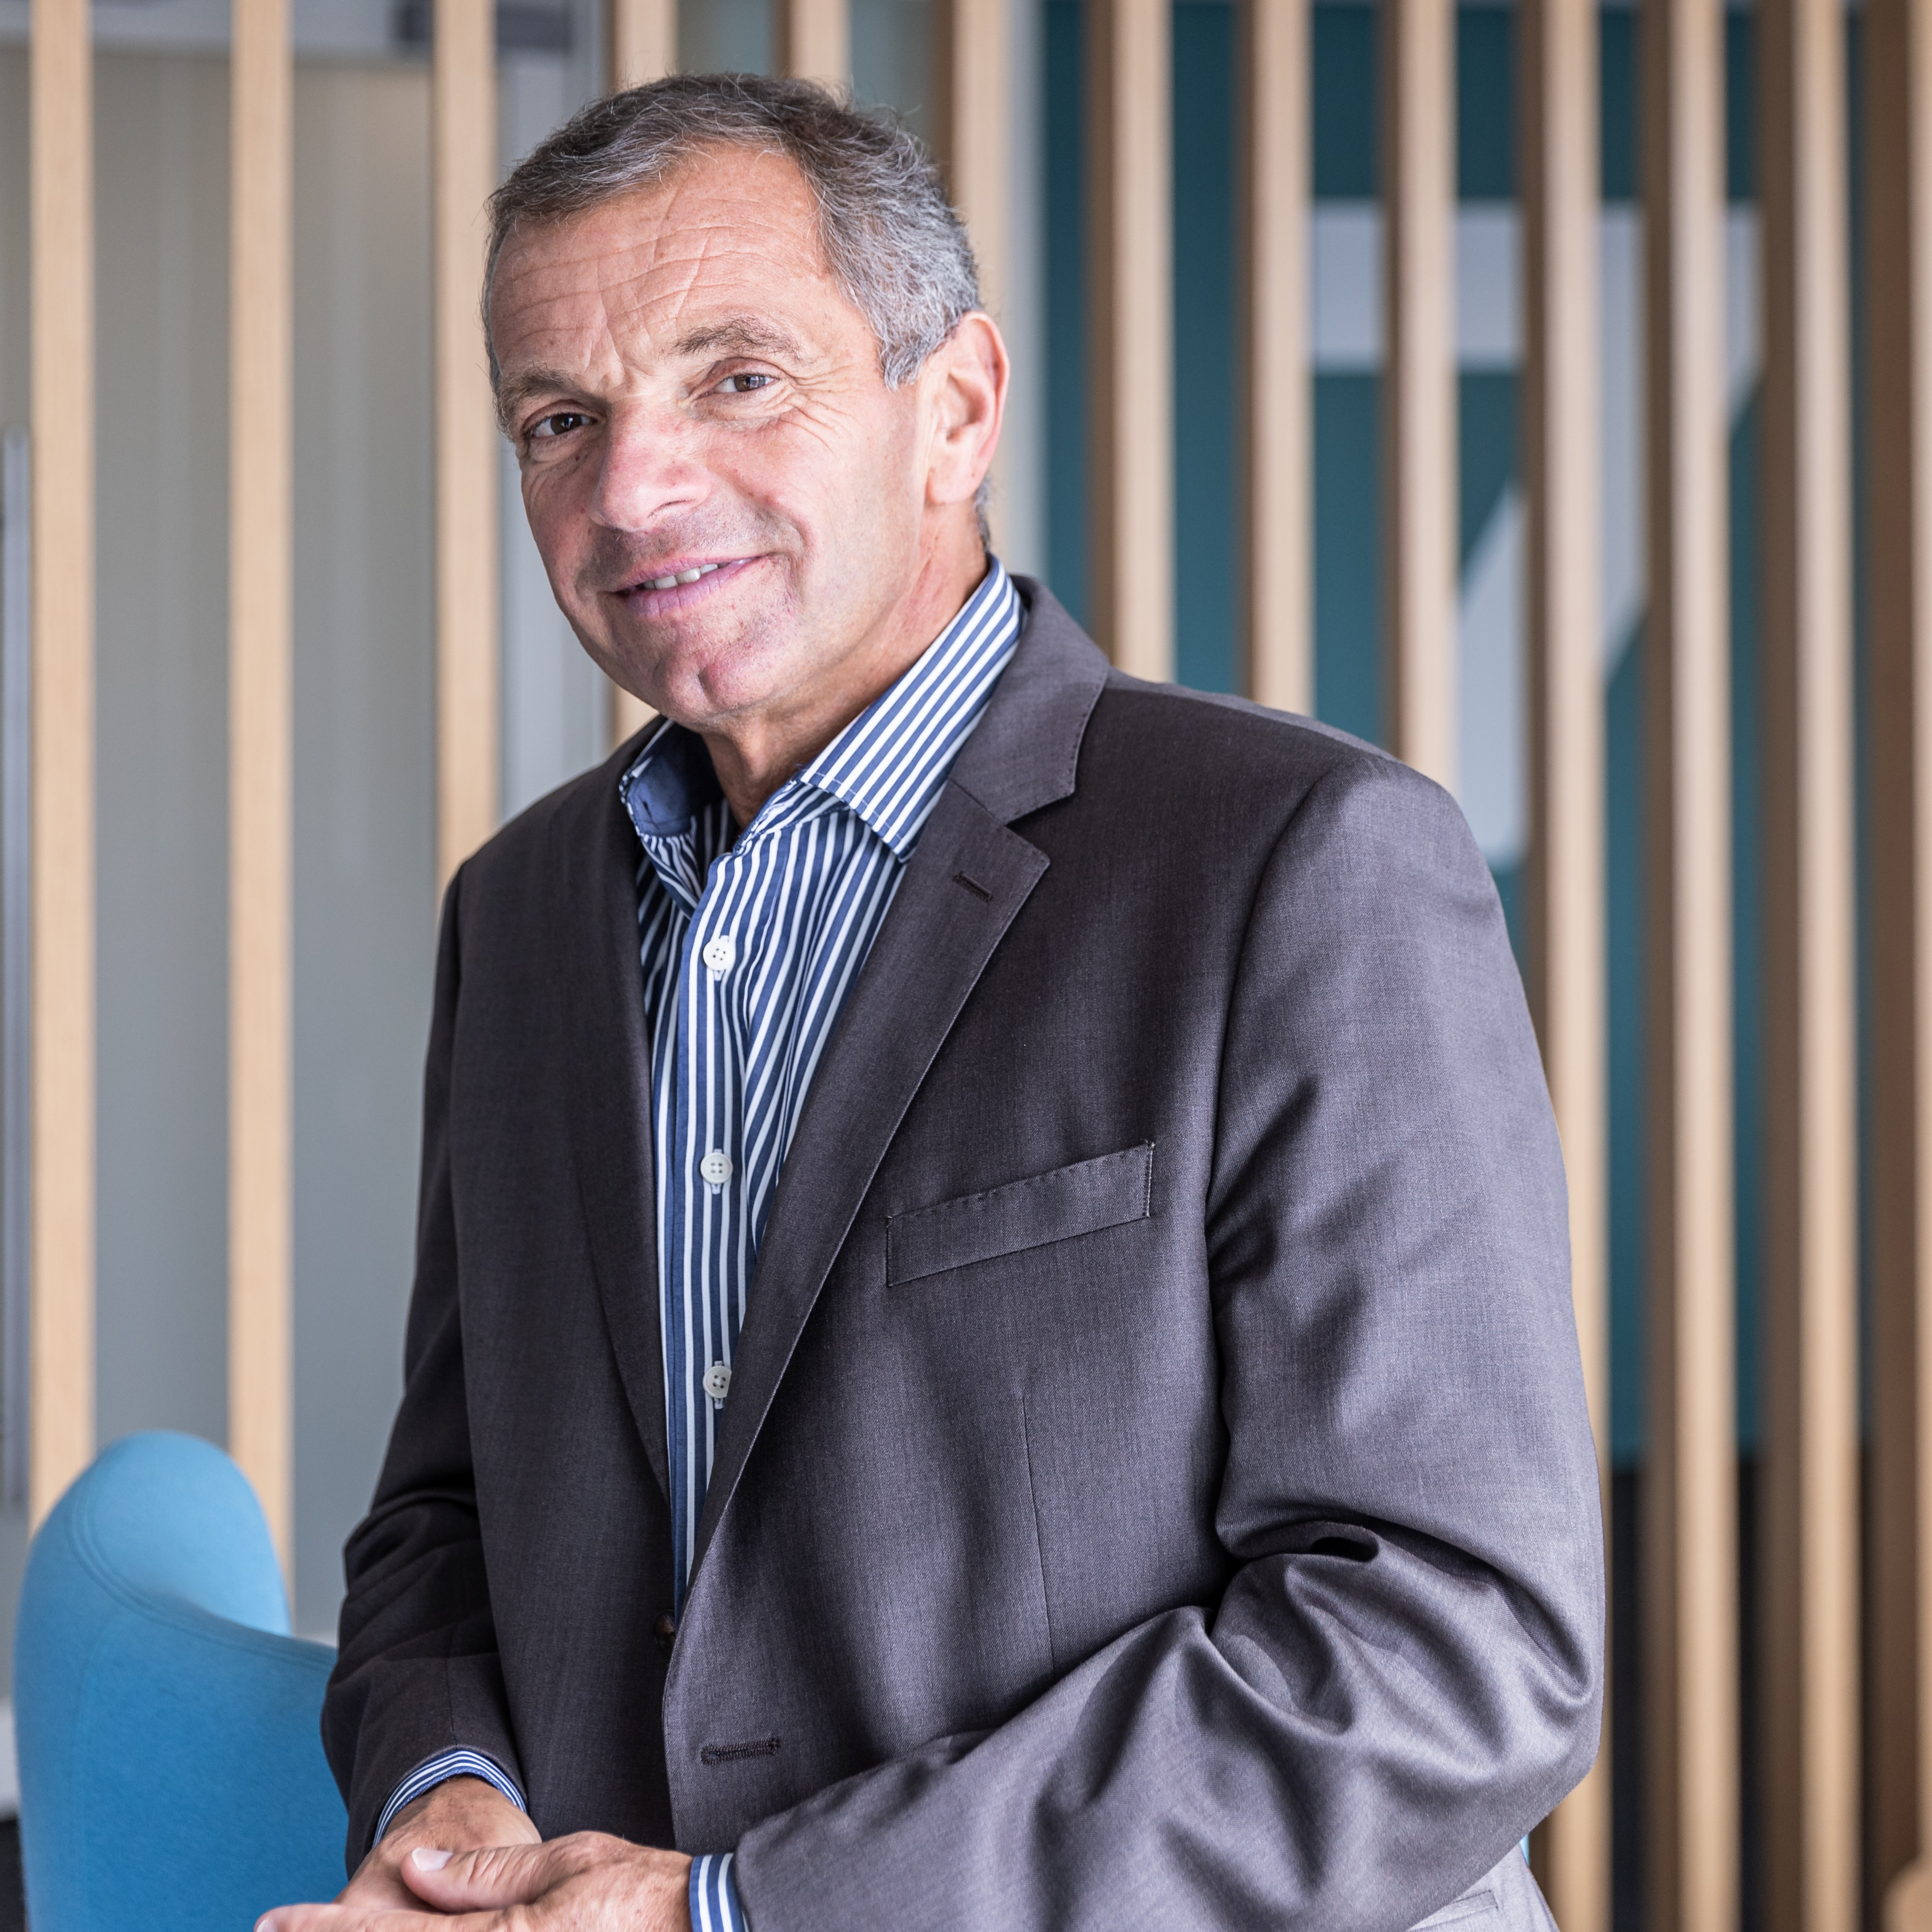
\includegraphics[width=0.7\textwidth]{img/hugues-meili.jpg}
    \caption{Hugues Meili}
  \end{minipage}
\end{figure}

\subsubsection{Création de l'entreprise}
Niji, qui signifie "arc-en-ciel" en japonais, est une entreprise co-fondée en septembre 2001 par Hugues Meili à Rennes. Niji est une ESN (Entreprise de service numérique) spécialisée dans le conseil, le design et le développement de solutions digitales pour des entreprises de toutes tailles. Depuis sa création, l'entreprise s'est imposée comme un acteur clé de la transformation numérique en France et à l'international.
\subsubsection{Positionnement et activités}
Niji se distingue par sa capacité à intervenir sur l'ensemble de la chaîne de valeur digitale. L'entreprise propose une large gamme de services adaptés aux besoins variés de ses clients. 
Tout d'abord, elle accompagne les entreprises dans la définition et la mise en œuvre de leur stratégie numérique. Cela inclut l'analyse des besoins métiers, l'identification des opportunités technologiques, et la conception de feuilles de route stratégiques alignées sur les objectifs de l'entreprise. Ce travail stratégique permet aux clients de mieux anticiper les évolutions du marché et de rester compétitifs.
\\\\
Ensuite, Niji excelle dans la conception de parcours utilisateurs innovants et intuitifs. Grâce à son expertise en design et en expérience utilisateur (UX/UI), l'entreprise crée des interfaces qui maximisent l'engagement des utilisateurs finaux. Cela inclut la réalisation de prototypes interactifs, des tests utilisateurs, et l'optimisation continue des interfaces pour garantir une expérience fluide et agréable.
\newpage
\noindent
Enfin, Niji développe et déploie des solutions technologiques sur mesure, intégrant les dernières innovations du marché. Cela comprend le développement d'applications web et mobiles, la mise en place de plateformes cloud, l'intégration de systèmes complexes, et l'automatisation des processus métiers. L'entreprise s'appuie sur des méthodologies agiles pour garantir une livraison rapide et de haute qualité, tout en s'adaptant aux besoins évolutifs des clients.
\\\\
En complément, Niji propose également des services de maintenance et de support technique pour assurer la pérennité des solutions déployées. Cela inclut la gestion des incidents, les mises à jour régulières, et l'accompagnement des équipes internes des clients pour une prise en main optimale des outils développés.
\\\\
Parmis les concurrents de Niji, on retrouve de grands groupe tels que Capgemini, Atos ou encore Sopra Steria, mais aussi des entreprises de taille intermédiaire comme Smile ou Devoteam. Niji se différencie par sa capacité à allier expertise technique et approche centrée sur l'utilisateur, ce qui lui permet de proposer des solutions innovantes et adaptées aux besoins spécifiques de chaque client. Niji dispose aussi aujourd'hui d'une solide réputation dans le secteur du développement numérique, grâce à la qualité de ses réalisations et à sa capacité à innover en permanence. L'entreprise est reconnue pour son approche collaborative et sa capacité à s'adapter aux évolutions rapides du marché technologique.
\subsubsection{Fonctionnement d'une ESN}
Une ESN (Entreprise de Services Numériques) est une entreprise spécialisée dans la fourniture de services informatiques et numériques. Elle intervient auprès de ses clients pour les accompagner dans leur transformation digitale, en proposant des solutions sur mesure adaptées à leurs besoins spécifiques. Le fonctionnement d'une ESN repose sur plusieurs éléments clés.
Tout d'abord, l'ESN recrute des experts dans divers domaines, tels que le développement logiciel, le design, la cybersécurité et le conseil. Ces experts sont ensuite affectés à des projets chez les clients, en fonction de leurs compétences et de leurs expériences. L'ESN agit en tant qu'intermédiaire entre ses collaborateurs et ses clients, en gérant les aspects administratifs, juridiques et financiers des missions.
\newpage
\subsubsection{Organisation interne}
Niji est structurée autour de plusieurs directions opérationnelles, chacune spécialisée dans un domaine particulier du numérique. Cette organisation permet de répondre efficacement aux besoins variés des clients et de favoriser la collaboration entre les équipes. Les principales directions sont :
\\
\begin{itemize}
    \item \textbf{DAF-SI} : Direction Administrative, Financière et Systèmes d'information
    \item \textbf{DRH} : Direction des Ressources Humaines
    \item \textbf{DCO} : Direction Commerciale
    \item \textbf{DCF} : Digital Consulting Firm (conseil stratégique et accompagnement à la transformation digitale)
    \item \textbf{DDA} : Digital Design Agency (design et expérience utilisateur)
    \item \textbf{DSF} : Digital Software Factory (développement logiciel, pôle Build et Run)
    \item \textbf{DST} : Digital Smart Technologies
    \item \textbf{DBS} : Digital Business Solutions
    \item \textbf{DCS} : Digital Cyber Security (Imineti by Niji, cybersécurité)
    \item \textbf{DDS} : Digital Data Solutions\\
\end{itemize}
\noindent
Chaque direction regroupe des experts dans son domaine et travaille en synergie avec les autres pour offrir des solutions complètes.
Par exemple, la DSF (Digital Software Factory) est responsable du développement des systèmes informatiques, tandis que la DDA se concentre sur le design et l’UX/UI.
La collaboration entre ces directions est facilitée par une culture d’entreprise basée sur la proximité, la transparence et l’innovation.
\\\\
L’entreprise valorise également la mobilité interne et la formation continue (ex : plateforme "Niji University"), permettant aux collaborateurs d’évoluer et de monter en compétences tout au long de leur parcours.
\subsubsection{Chiffres clés}
En 2025, Niji compte plus de 1400 collaborateurs répartis sur plusieurs sites en France et à l'international. L'entreprise, créée en 2001, réalise un chiffre d'affaires de 142 millions d'euros sur l'année 2024, avec une croissance de 20\% de son CA sur 5 ans, témoignant de sa solidité financière et de sa capacité à répondre aux attentes du marché.
\\\\
Niji accompagne plus de 300 clients, parmi lesquels figurent de grands groupes internationaux et nationaux, ainsi que des ETI et PME implantées sur l'ensemble des territoires. Cette diversité de clientèle illustre la capacité de l'entreprise à s'adapter à des besoins variés et à intervenir sur des projets d'envergure comme sur des missions plus ciblées.
\\\\
L'entreprise adresse plus de 25 secteurs d’activité, ce qui en fait un acteur multi-sectoriel reconnu. Niji intervient notamment dans les domaines de la banque, de l’assurance, des télécommunications, de l’énergie, du transport, de la distribution, de la santé, ou encore du secteur public, renforçant ainsi son expertise et sa polyvalence.
\\\\
Niji est présente dans dix sites en France, notamment à Rennes (siège social), Paris, Lyon, Lille, Nantes, Angers, Bordeaux et Nice. À l’international, l’entreprise dispose de bureaux à Singapour et Casablanca, renforçant ainsi sa dimension globale et sa capacité à accompagner des clients de toutes tailles, y compris des grands groupes internationaux. Récemment, Niji a également ouvert un nouveau site à Madrid, en Espagne, suite au rachat de l'entreprise Neo9, marquant une étape importante dans sa stratégie d’expansion européenne.
\subsubsection{La démarche RSE de Niji}
Niji s'engage activement dans une démarche de responsabilité sociétale des entreprises (RSE). Cela se traduit par des actions concrètes en faveur du développement durable, de la diversité et de l'inclusion. L'entreprise soutient également des initiatives locales et encourage ses collaborateurs à s'impliquer dans des projets solidaires.
\\\\
Dans une démarche de développement durable, Niji s'efforce chaque année de réduire son empreinte carbone. L'entreprise met en place des actions concrètes pour limiter la production de CO2 liée à ses activités, que ce soit par l'optimisation des déplacements professionnels, la mise en place du télétravail, la sensibilisation des collaborateurs aux éco-gestes ou encore l'amélioration de l'efficacité énergétique de ses infrastructures. Cette volonté de diminuer progressivement la fabrication de CO2 s'inscrit dans la politique RSE de Niji et témoigne de son engagement en faveur de la transition écologique.

\subsubsection{Perspectives d'avenir}

Niji ambitionne de poursuivre sa croissance en renforçant sa présence sur les marchés existants et en explorant de nouvelles opportunités.
Niji est en constante recherche de nouveaux talents pour accompagner sa croissance et répondre aux besoins variés de ses clients. L'entreprise recrute régulièrement des experts dans des domaines diversifiés, tels que le développement logiciel, la cybersécurité, le design UX/UI, ou encore l'intelligence artificielle. Cette stratégie de recrutement permet à Niji de rester à la pointe des innovations technologiques et d'offrir des solutions adaptées aux enjeux actuels.
\subsection{Le site de Rennes}
\subsubsection{Spécificités du site}
C'est en Bretagne, à Rennes, que Niji a ouvert sa première antenne en 2001. L'antenne Rennaise de Niji est aujourd'hui l'une des plus importantes de l'entreprise, avec plus de 300 collaborateurs. L'antenne Rennaise est un pôle d'excellence pour Niji, qui y développe des projets innovants et accompagne des clients de renom dans leur transformation digitale. Avec l'évolution de l'entreprise et les nouveaux bureaux ouverts dans les différentes villes de France, notamment à Paris, les bureaux bretons sont restés le siège social de l'entreprise notamment pour des raisons historiques mais surtout pour l'amour de la Bretagne du fondateur.
\\\\
Les bureaux de Niji à Rennes sont situés à EuroRennes, une nouvelle zone d'activité dynamique, à proximité de la gare et du centre-ville. S'étalant sur 3 étages, les locaux sont modernes et spacieux, offrant un cadre de travail agréable et stimulant pour les collaborateurs. Les bureaux Rennais sont équipés de salle de réunions, de cabines insonorisées, d'un espace de restauration avec une terrasse extérieure. Les espaces de travail sont modulables et permettent aux équipes de s'organiser selon leur besoins. 
\subsubsection{Imineti by Niji}
\begin{wrapfigure}{l}{0.32\textwidth}
    \centering
    
\includegraphics[width=0.85\linewidth]{img/imineti.jpg} 
    \caption{Logo de Imineti by Niji}
    \label{fig:wrapfig}
\end{wrapfigure}
Imineti by Niji est une branche de l'entreprise Niji spécialisée dans la gestion des risques numériques et la cybersécurité. Elle combine conseil en cybersécurité et expertise technique pour aider les entreprises à définir et mettre en œuvre des stratégies de sécurité efficaces. Imineti by Niji accompagne ses clients tout au long du processus, de l'analyse des risques et des tests d'intrusion jusqu'à la présentation des recommandations devant les comités de direction. L'objectif est de fournir une vision cohérente et à long terme de la sécurité, en aidant les entreprises à formaliser et à appliquer des règles de sécurité adaptées à leurs besoins.
\\
Imineti by Niji est localisé à Rennes, au sein de l'antenne Rennaise de Niji. Pour des raisons de sécurité et de confidentialité, l'accès aux bureaux d'Imineti est restreint. Si une personne non autorisée souhaite entrer dans les locaux d'Imineti, elle doit remplir une feuille en spécifiant son identité, son heure d'arrivée et de départ. Ainsi, les équipes d'Imineti peuvent savoir qui est présent dans les locaux à tout moment. De plus, l'accès aux bureaux d'Imineti est sécurisé par des badges magnétiques, ce qui permet de contrôler les entrées et sorties des personnes autorisées.
\newpage
\subsection{Le département DSF (Digital Software Factory)}
Durant mon contrat d'apprentissage avec Niji, j'ai intégré la direction opérationnelle DSF (Digital Software Factory). Ce département est en charge du développement des systèmes informatiques des clients de Niji.
\\\\
Le département est constitué de deux pôles principaux : le pôle "Build" et le pôle "Run". Le pôle "Build" est en charge de la conception et du développement de solutions digitales pour les clients de Niji, tandis que le pôle "Run" assure la maintenance et l'exploitation de projets déjà déployés et en production. Le pôle "Run" est également en charge de la gestion des incidents et des demandes de support technique.
\\\\
Les clients du département DSF sont variés, allant des grandes entreprises aux PME, et couvrent de nombreux secteurs d'activité. 
Alban GRÉAU, mon tuteur, est nottament architecte solution pour les projets de développement d'une application mobile de e-commerce pour Lacoste ainsi que pour un projet de la banque BNP.
\subsection{Mon rôle en tant qu’alternant}
\subsubsection{Poste et missions}
Durant mon contrat d'apprentissage avec Niji, j'ai intégré la direction opérationnelle DSF (Digital Software Factory) et ai été affecté au poste de "Ingénieur solutions".
Je n'ai pas intégré d'équipe existante en particulier. En effet, j'ai été affecté à un projet interne de l'entreprise dont le développement n'avait pas encore débuté. Aucune équipe n'a donc été formée pour ce projet. Cependant, j'ai eu l'occasion de travailler avec plusieurs collaborateurs de Niji pour la mise en place de ce projet et son développement :
\paragraph{Alban GRÉAU} est le responsable du projet NijiSkills. Il a été mon tuteur durant mon année d'alternance et m'a accompagné tout au long de mon parcours chez Niji. Alban est architecte solution à Niji Rennes, et possède une solide expérience dans la gestion de projets digitaux. Il a su me guider et me conseiller dans mes missions, tout en me laissant une certaine autonomie pour développer mes compétences et donner mon avis sur certaines solutions.
\paragraph{Olivier DELALANDE} est un développeur React au sein de l'équipe DSF à Niji Paris. Il m'a rejoint sur le projet NijiSkills en tant que développeur en Avril 2025 afin d'apporter son expertise technique et de m'aider à développer le projet. Olivier a une forte expérience dans le développement d'application web avec React et a su me guider quant aux bonnes pratiques de développement. Il est intervenu notamment sur la partie de synchronisation des compétences entre l'application Nijskills et DoYouBuzz, une plateforme de création de CV en ligne.
\\\\
Ma mission principale au sein de Niji, pour ma période d'alternance, à été le développement de l'application interne NijiSkills. Cette application a pour but de centraliser les compétences des collaborateurs de Niji, de les aider à se former en leur proposant des parcours de compétences à acquérir pour évoluer dans leur carrière, et de les accompagner dans leur montée en compétences. NijiSkills est un projet ambitieux qui vise à améliorer la gestion des compétences au sein de l'entreprise et à favoriser le développement professionnel des collaborateurs.
\subsubsection{Objectifs professionnels de l’alternance}
Au début de mon alternance chez Niji, je voulais découvrir le fonctionnement d’une grande entreprise. Après une expérience dans une petite structure, il était important pour moi de comprendre comment s’organisent les équipes, comment se passe la communication entre les différents services et comment sont gérés les projets à grande échelle. Cette immersion m’a permis d’avoir une vision plus large du secteur du numérique et de découvrir les enjeux et les défis auxquels sont confrontées les grandes entreprises.
\\\\
Un autre objectif était de renforcer mes compétences techniques en travaillant sur de nouvelles technologies. Le développement de l’application NijiSkills m’a permis d’apprendre de nouveaux outils et frameworks, tout en les utilisant directement dans un contexte professionnel. Cette expérience m’a poussé à sortir de ma zone de confort, à chercher des solutions par moi-même et à demander de l’aide à mes collègues si besoin.
J'ai donc dû apprendre ces technologies directement en développant l'application NijiSkills, sans passer par la réalisation de projets d'entraînement ou de tests préalables, ce qui m'a permis d'acquérir des compétences concrètes en situation réelle.
Mais aussi, j'ai pu approfondir mes connaissances en React, TypeScript et Node.js, des technologies que je n'avais pas eu l'occasion d'utiliser en profondeur auparavant.
\\\\
Enfin, l’un des objectifs majeurs de mon alternance était de pouvoir poursuivre ma carrière chez Niji à l’issue de cette expérience, en obtenant une proposition de contrat. J’ai donc mis un point d’honneur à démontrer mon sérieux, mon implication et ma capacité à mener à bien un projet complet, afin de convaincre l’entreprise de m’accorder sa confiance pour la suite de mon parcours professionnel.
\newpage
\section{Présentation de la mission : développement de NijiSkills}
\subsection{Contexte du projet}
Dans cette section, je vais présenter le contexte dans lequel s’inscrit ma mission au sein de Niji, ainsi que les objectifs qui ont guidé le développement de l’application NijiSkills. Comprendre l’environnement, les enjeux et les attentes liés à ce projet est essentiel pour appréhender les choix techniques et organisationnels qui ont été faits tout au long de la mission. Cette présentation permettra de mettre en lumière les besoins auxquels l’application devait répondre, les contraintes rencontrées, ainsi que la démarche adoptée pour concevoir une solution adaptée aux spécificités de l’entreprise et de ses collaborateurs.
\subsubsection{Origine du besoin}
L'origine du besoin pour le projet NijiSkills provient d'abord du constat d'Alban GRÉAU, architecte solution et responsable du projet, qu'il devenait compliqué d'évaluer un candidat lors d'un entretien avec une simple grille de questions et une note pour chaque question. Cette méthode, bien que répandue, montrait rapidement ses limites : elle ne permettait pas de refléter fidèlement la diversité et la profondeur des compétences d'un candidat, ni de prendre en compte les parcours d'apprentissage ou les évolutions de carrière possible. Face à cette difficulté, Alban a exprimé le besoin de disposer d'un outil plus structurant et plus précis pour cartographier les compétences, suivre leur évolution et faciliter l'évaluation lors des entretiens. Ce constat a servi de point de départ à la réflexion autour de la création d'une application dédiée, capable de centraliser et de valoriser les compétences des collaborateurs tout en offrant une meilleure visibilité sur les axes de progression possibles.
\\\\
Dans ce contexte, la mise en place d’un outil interne permettant de cartographier les
compétences, de faciliter la montée en compétences des équipes et d’optimiser l’affectation
des collaborateurs sur les projets. L’objectif était également de proposer un accompagnement
personnalisé aux collaborateurs dans leur évolution professionnelle, en leur offrant une
meilleure visibilité sur les compétences à acquérir pour atteindre leurs objectifs de carrière.
\\\\
Le projet s’inscrit donc dans une démarche d’amélioration continue des processus RH
et de développement des talents, tout en répondant à des enjeux opérationnels concrets :
mieux connaître les expertises internes, anticiper les besoins en formation, et renforcer
l’attractivité de Niji en tant qu’employeur. Le développement de NijiSkills s’est appuyé
sur une collaboration étroite entre les équipes techniques, les ressources humaines et les
managers, afin de concevoir une solution adaptée aux attentes de l’ensemble des parties
prenantes.
\subsubsection{Objectifs de l’application}
L’application NijiSkills vise avant tout à centraliser l’ensemble des compétences des collaborateurs de Niji dans un outil unique. Cette centralisation permet de disposer d’une cartographie précise et à jour des expertises présentes au sein de l’entreprise. Grâce à cette visibilité, il devient plus simple pour les managers et les équipes RH d’identifier les forces internes, de repérer les besoins en formation, et d’optimiser l’affectation des collaborateurs sur les projets en fonction de leurs compétences réelles.
\\\\
Un autre objectif majeur du projet est d’explorer et d’expérimenter de nouvelles technologies qui n’étaient pas encore utilisées chez Niji. Le choix de Next.js pour le développement du front-end et de l’API, associé à TailwindCSS pour le design et à Prisma comme ORM pour la gestion de la base de données PostgreSQL, s’inscrit dans une démarche d’innovation technique. Cette volonté d’adopter des outils modernes permet non seulement d’enrichir la culture technologique de l’entreprise, mais aussi de préparer l’équipe à de futurs projets nécessitant ces compétences.
\\\\
Enfin, NijiSkills ambitionne de proposer un accompagnement personnalisé aux collaborateurs dans leur évolution professionnelle. En offrant une vision claire des compétences à acquérir et des parcours de progression possibles, l’application facilite la montée en compétences et encourage le développement continu. Elle contribue ainsi à renforcer l’attractivité de Niji en tant qu’employeur et à fidéliser les talents en leur offrant des perspectives d’évolution concrètes et adaptées à leurs aspirations.
\subsubsection{Contraintes techniques et fonctionnelles}
Il n’existe pas de contrainte technique majeure imposée par l’environnement ou le contexte du projet NijiSkills. Les contraintes rencontrées sont principalement issues de choix délibérés réalisés par Alban GRÉAU, responsable du projet, dans une démarche d’exploration de nouvelles technologies et de méthodes de développement. L’objectif était de sortir des sentiers battus et d’expérimenter des outils et frameworks encore peu utilisés chez Niji, afin d’enrichir la culture technique de l’équipe et d’ouvrir de nouvelles perspectives pour les futurs projets.
\\\\
Ainsi, le choix de la stack technique (Next.js, TailwindCSS, Prisma, PostgreSQL) n’a pas été dicté par des exigences externes ou des limitations techniques, mais bien par la volonté de tester des solutions innovantes et de se confronter à des problématiques inédites. Cette approche a permis de découvrir de nouvelles façons de concevoir et de développer une application complète, tout en favorisant l’apprentissage continu et l’adaptabilité.
\\\\
Il existait toutefois une contrainte technique importante : il fallait proposer une visualisation des compétences sous forme de "carte", à la manière de ce que propose le site roadmap.sh. Cela impliquait de mettre en place un "canvas" interactif permettant d’afficher, de relier et de manipuler graphiquement les différentes compétences, afin d’offrir une vue d’ensemble claire et intuitive. Ce besoin a fortement orienté les choix techniques et la conception de l’interface utilisateur.
\\\\
En conséquence, les contraintes du projet étaient davantage organisationnelles et pédagogiques que techniques. Il s’agissait de s’approprier rapidement des technologies inconnues, de mettre en place des bonnes pratiques de développement dans un contexte d’apprentissage, et de garantir la qualité du code tout en assurant l’avancement du projet. Ce cadre a offert une grande liberté dans la conception de l’application, tout en posant le défi de structurer le projet de manière efficace et pérenne.
\subsection{Cadrage du projet}
\subsubsection{Méthodologie utilisée}
Habituellement, Niji travaille en mode agile, en mettant en place des méthodologies telles que Scrum ou Kanban, avec des équipes projet complètes, des rituels réguliers (sprints, daily meetings, rétrospectives) et un suivi itératif de l'avancement. Cependant, dans le cadre du développement de NijiSkills, le contexte était particulier : n'étant pas intégré à une équipe projet complète et travaillant principalement en autonomie, il n'a pas été pertinent d'appliquer une méthodologie agile classique. Pour assurer un suivi rigoureux de l'avancement et de la priorisation des tâches, l'outil Jira a été utilisé tout au long du projet. Jira a permis de lister, organiser et suivre l'ensemble des tâches à réaliser. Cet usage a facilité la communication avec mon tuteur et les intervenants ponctuels, tout en offrant une visibilité claire sur la progression du développement de l'application.
\\
\begin{figure}[H]
  \centering
  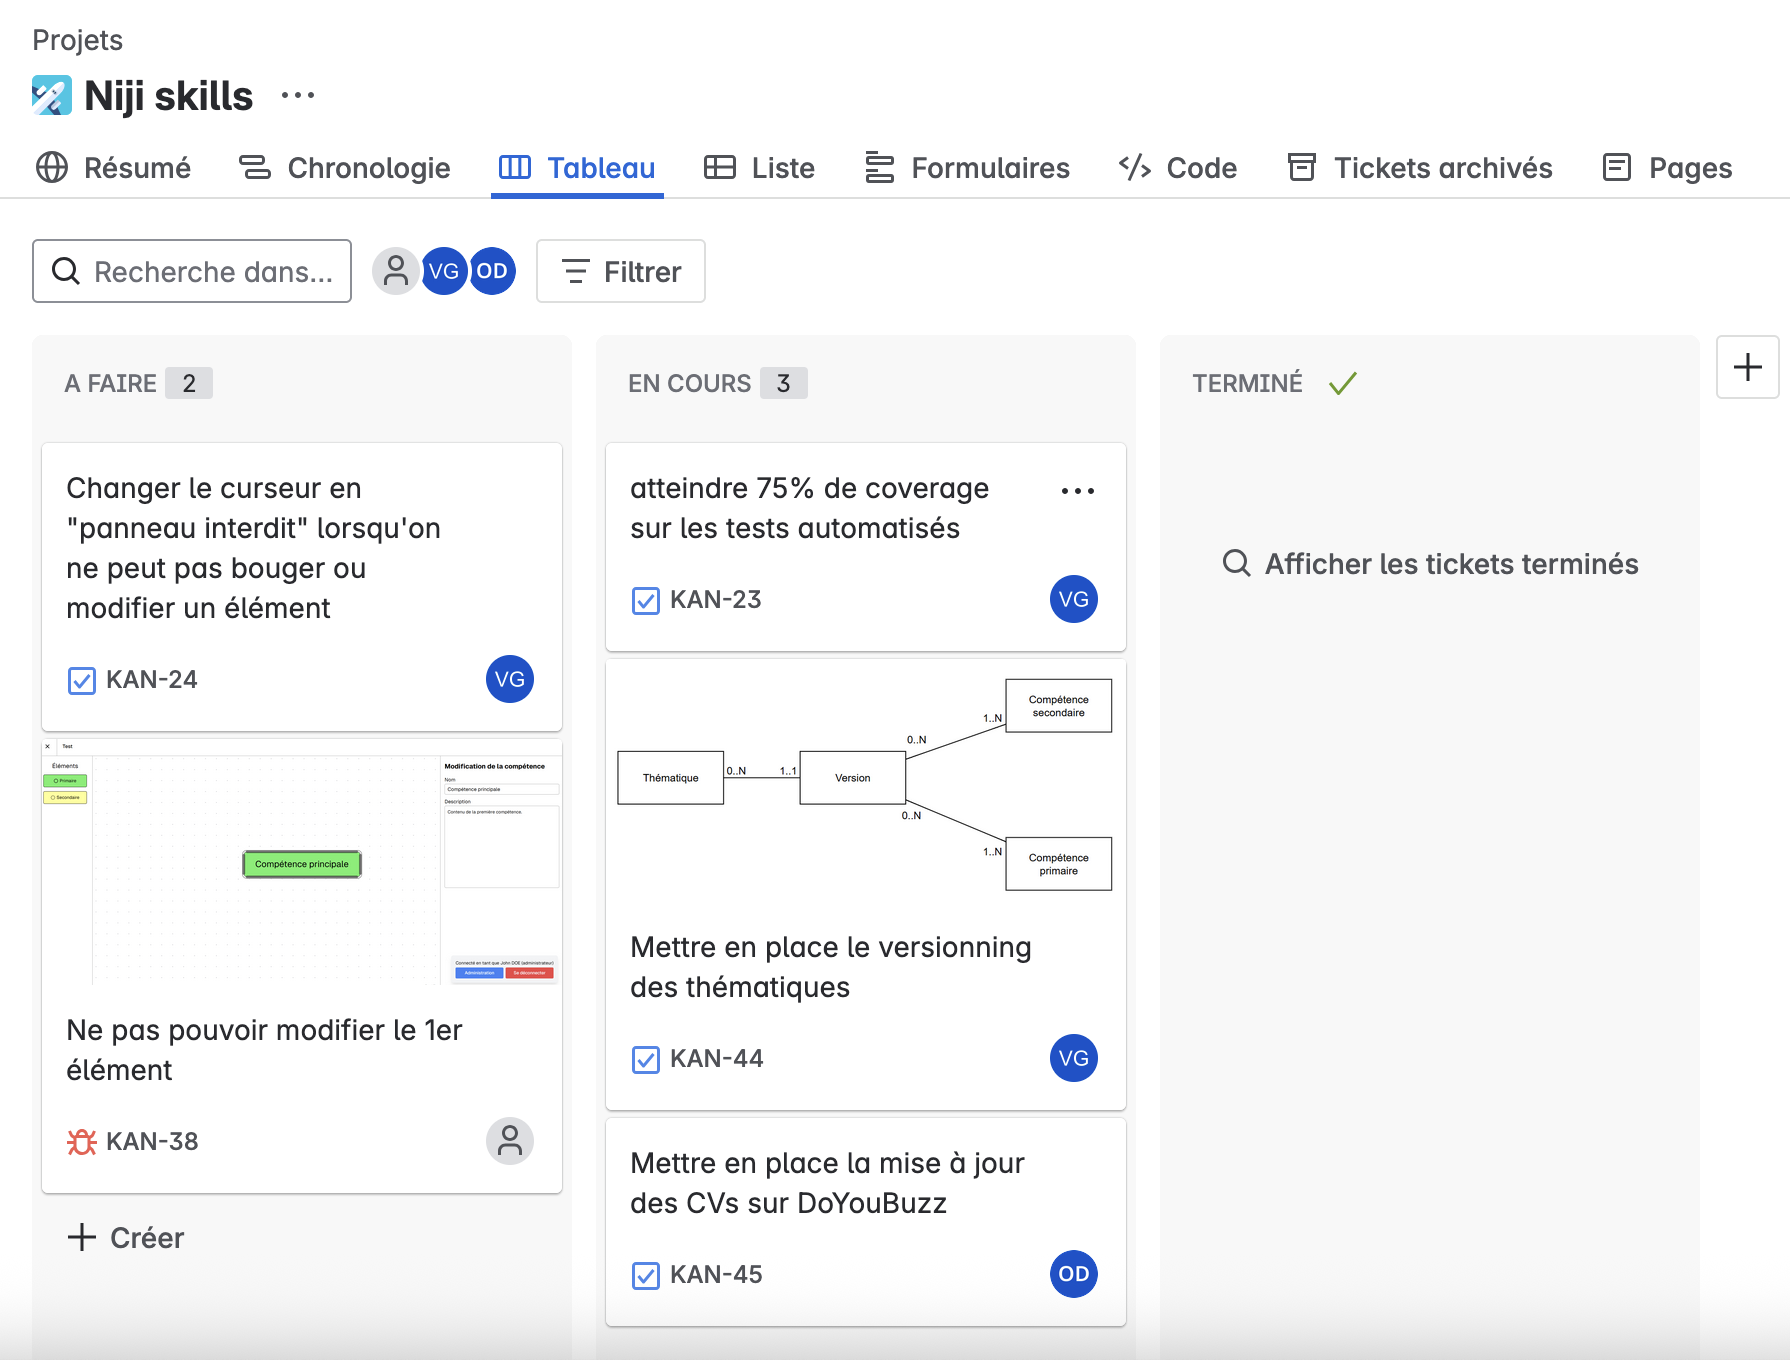
\includegraphics[width=0.8\textwidth]{img/jira.png}
  \caption{Exemple d'utilisation de Jira pour le suivi des tâches du projet NijiSkills}
\end{figure}

\subsubsection{Planification et priorisation des tâches}
Le découpage des tâches du projet NijiSkills s’est fait par paliers de réalisation, chaque tâche correspondant à une fonctionnalité majeure de l’application. Nous avons ainsi débuté par les fondations techniques indispensables, telles que la mise en place du SSO Microsoft, la connexion à la base de données, l’intégration de la CI (Continuous Integration) et l’ajout des premiers tests unitaires avec Jest. Ce premier palier a permis de garantir un socle technique robuste et sécurisé, sur lequel les développements ultérieurs ont pu s’appuyer.
\\\\
Une fois ces éléments essentiels en place, le découpage des tâches a évolué pour accompagner la montée en complexité de l’application. Chaque nouvelle tâche représentait alors soit l’ajout d’une nouvelle fonctionnalité (feature), soit une amélioration ou une correction du fonctionnement existant. Par exemple, la gestion du versionning des thématiques, l’ajout du rôle manager, ou encore la mise en place de la gestion des utilisateurs par les managers ont constitué des étapes importantes dans l’évolution du projet. Ce découpage progressif a permis d’avancer de manière structurée, en validant chaque étape avant de passer à la suivante.
Il est important de souligner que les tâches n’étaient pas associées à des dates limites strictes. Au lieu d’imposer des deadlines fixes, nous avons préféré organiser les tâches selon leur niveau d’urgence et leur impact sur l’avancement global du projet. Cette approche a permis de rester flexible et de s’adapter aux imprévus, tout en assurant que les priorités les plus critiques étaient traitées en premier. La classification par urgence a également facilité la communication avec les parties prenantes et permis de réagir rapidement en cas de besoin.
\\\\
En résumé, la planification du projet s’est appuyée sur un découpage par paliers fonctionnels, une priorisation par urgence plutôt que par échéance, et une adaptation continue aux besoins et aux retours des utilisateurs. Cette organisation a favorisé la progression régulière du développement tout en maintenant une grande réactivité face aux évolutions du projet.
\subsubsection{Collaboration inter-équipes}
La grande force de Niji est qu'elle possède de nombreux pôles d'expertise, ce qui permet de collaborer avec des experts dans différents domaines. Ainsi, pour le développement de l'application NijiSkills, j'ai pu bénéficier de l'expertise d'Alban GRÉAU, mon tuteur. Alban a su me guider dans la conception et le développement de l'application, en m'apportant son expérience et ses conseils sur les choix techniques à adopter. J'ai aussi pu travailler avec Olivier DELALANDE, un développeur React de l'équipe DSF à Niji Paris. Olivier a apporté son aide technique et m'a aidé à développer certaines fonctionnalités de l'application, notamment la synchronisation des compétences entre NijiSkills et DoYouBuzz.
\\\\
J'ai aussi pu travailler avec l'équipe chargée des tests à Niji. Premièrement, Antoine VALLERY, un testeur de l'équipe DSF à Rennes, a testé plusieurs aspects globaux de l'application Nijiskills grâce à une documentation utilisateur que j'ai rédigée. Il a pu ainsi vérifier que l'application répondait aux besoins fonctionnels et qu'elle était conforme aux attentes des utilisateurs. 
\\\\
J'ai aussi pu discuté avec Tanguy MICHEL pour la mise en place de tests E2E \footnote{End to end:  tests automatisés qui valident le bon fonctionnement d’une application dans son ensemble, en simulant le parcours complet d’un utilisateur final } avec Playwright. Tanguy est un développeur de l'équipe DSF à Rennes, et il m'a aidé à comprendre comment mettre en place des tests automatisés pour vérifier le bon fonctionnement de l'application dans son ensemble. Ces tests permettront de s'assurer que les différentes fonctionnalités de NijiSkills fonctionnent correctement et que l'application est stable. Il m'a aussi expliquer comment mettre en place Playwright dans le projet, et comment l'utiliser pour écrire des tests E2E.
\\\\
J'ai aussi eu à contacter Dimitri GOULIARMIS, un developpeur Flutter de l'équipe DSF à Rennes, pour qu'il puisse créer une première thématique "Flutter" de test pour pouvoir l'utiliser pendant un prochain entretien.

\subsection{Architecture technique}
\subsubsection{Choix de la stack}
\begin{figure}[H]
  \centering
  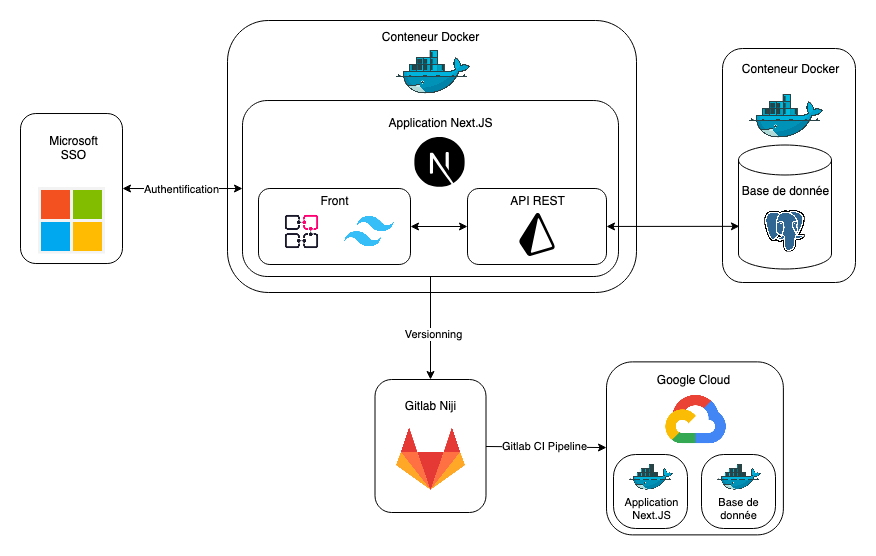
\includegraphics[width=0.9\textwidth]{img/archi.png}
  \caption{Architecture du projet}
\end{figure}

L’architecture technique de l’application NijiSkills repose sur une stack moderne et performante. Le choix de Next.js avec TypeScript permet de bénéficier d’un framework robuste pour le développement à la fois du front-end et de l’API, offrant ainsi une cohérence et une maintenabilité accrues du code. L’utilisation de TailwindCSS facilite la création d’interfaces utilisateur réactives et personnalisées, tout en accélérant le processus de développement grâce à ses classes utilitaires. La base de données PostgreSQL, reconnue pour sa fiabilité et ses performances, est gérée via l’ORM Prisma, qui simplifie les interactions avec la base et améliore la productivité des développeurs. Enfin, l’ensemble de l’application est conteneurisé avec Docker, ce qui garantit la portabilité, la reproductibilité des environnements et facilite le déploiement sur différents serveurs ou plateformes cloud. Cette combinaison de technologies assure à la fois flexibilité, évolutivité et sécurité pour le projet.
\newpage
\subsubsection{Authentification SSO Microsoft}
L’application NijiSkills étant destinée exclusivement aux collaborateurs de Niji, il était impératif de restreindre l’accès à la plateforme afin de garantir la confidentialité des données et d’éviter toute utilisation non autorisée. Pour répondre à cette exigence, la mise en place d’une authentification SSO (Single Sign-On) via Microsoft a été choisie. Cette solution permet de s’assurer que seuls les salariés disposant d’un compte Microsoft professionnel Niji peuvent se connecter à l’application, consulter ou compléter leurs compétences. L’authentification SSO offre également une expérience utilisateur fluide, en évitant la multiplication des identifiants et mots de passe, tout en renforçant la sécurité globale de l’accès à l’outil.
\\\\
La mise en place d’une connexion SSO avec Microsoft nécessite plusieurs étapes techniques. Tout d’abord, il faut enregistrer l’application NijiSkills auprès de l’Azure Active Directory (Azure AD) de Niji, en créant une nouvelle application dans le portail Azure. Cette opération permet d’obtenir un identifiant client (Client ID) et un secret d’application (Client Secret), qui serviront à authentifier l’application auprès des services Microsoft. Ensuite, il convient de configurer les redirections d’URL autorisées, afin que Microsoft puisse renvoyer l’utilisateur vers l’application après authentification.
\begin{figure}[H]
  \centering
  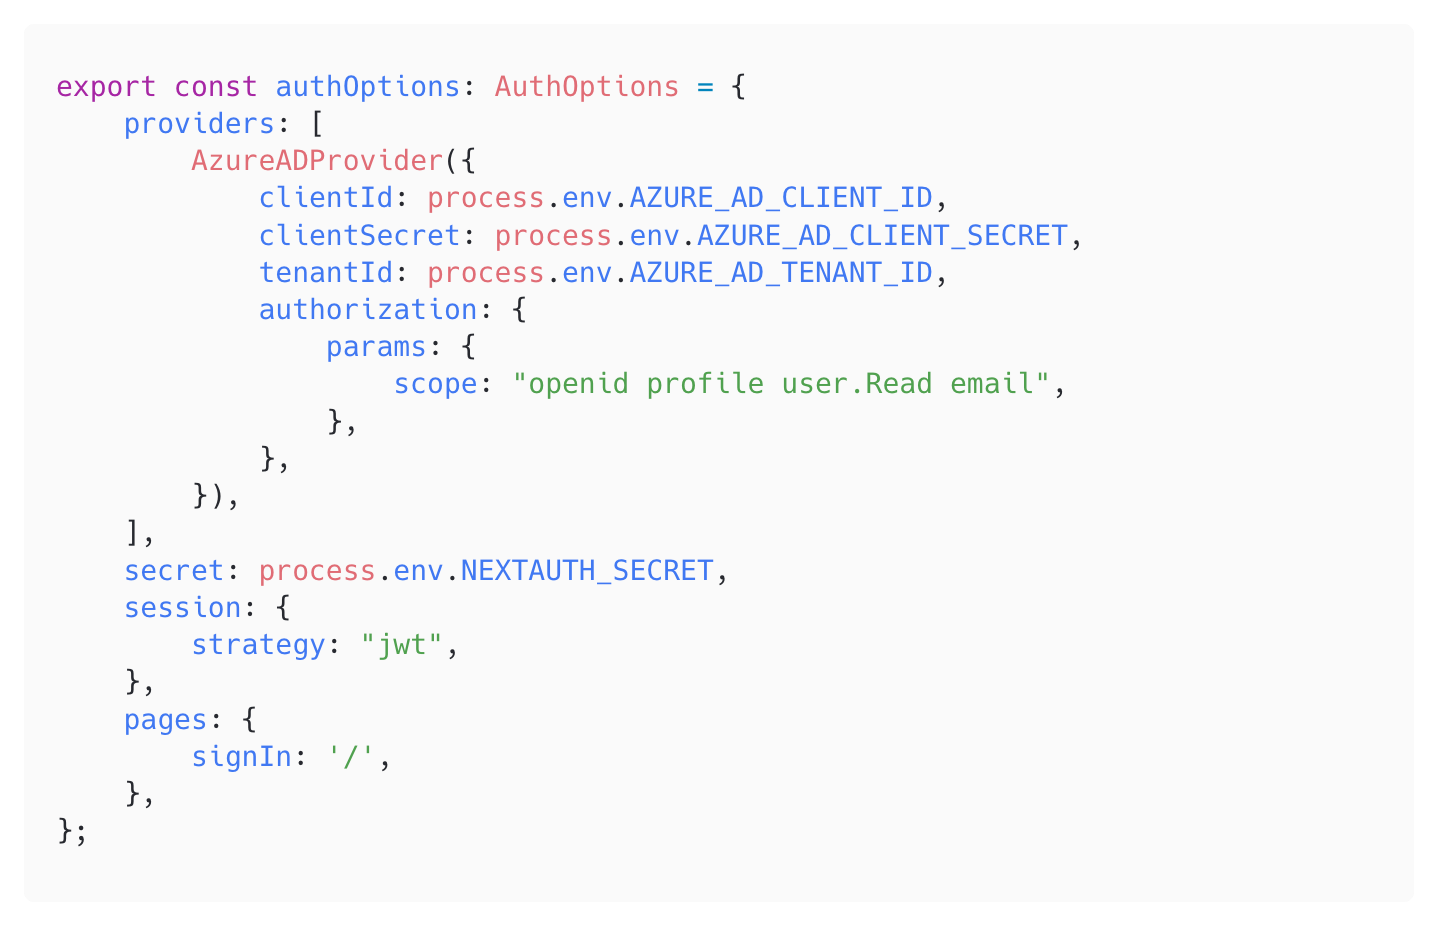
\includegraphics[width=0.75\textwidth]{img/code-auth.png}
  \caption{Exemple de code pour l'intégration de l'authentification SSO Microsoft avec NextAuth.js}
\end{figure}
\noindent
Côté application, il est nécessaire d’intégrer une bibliothèque compatible avec le protocole OAuth 2.0 et OpenID Connect, comme \texttt{next-auth} pour Next.js et de configurer les options avec les identifiants récupérer précedemment. Cette bibliothèque facilite la gestion du flux d’authentification, la récupération des informations de l’utilisateur (nom, email, etc.) et la gestion des sessions. Lorsqu’un utilisateur tente de se connecter, il est redirigé vers la page de connexion Microsoft, où il doit s’authentifier avec ses identifiants professionnels. Une fois l’authentification validée, Microsoft renvoie un jeton d’accès (access token) à l’application, qui peut alors vérifier l’identité de l’utilisateur et lui accorder l’accès à la plateforme.
\\\\
Enfin, côté serveur, une fois que l'utilisateur est authentifié, on vérifie que le compte existe en base de données. Si le compte n'existe pas, on le crée automatiquement avec les informations récupérées depuis Microsoft (nom, prénom, email). Cela permet de garantir que tous les collaborateurs de Niji peuvent accéder à l'application sans avoir à créer manuellement un compte.
\subsubsection{Hébergement et déploiement}
Le déploiement de l’application est entièrement automatisé grâce à une pipeline d’intégration continue (CI) mise en place sur GitLab. Cette pipeline repose sur une configuration standardisée, dite « universelle », adoptée pour l’ensemble des projets de Niji. Cette approche garantit une cohérence et une qualité constante lors des déploiements, tout en facilitant la maintenance et l’évolution des différents projets.
\\
\begin{figure}[H]
  \centering
  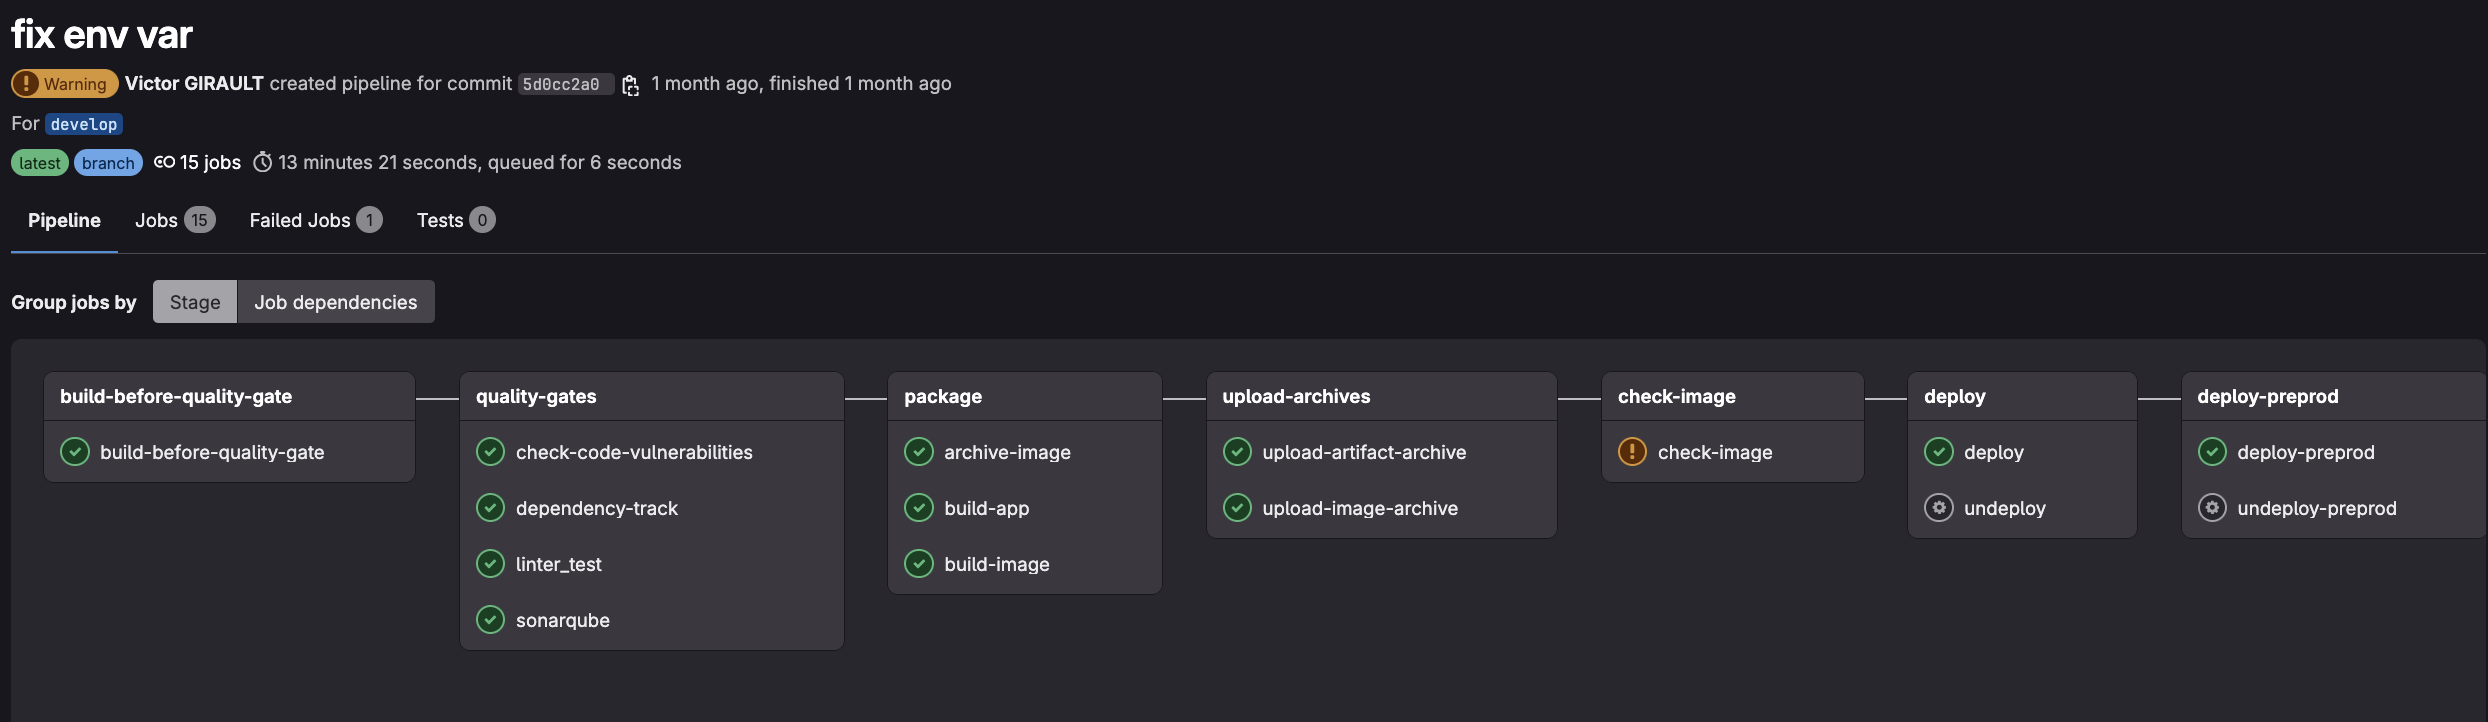
\includegraphics[width=\textwidth]{img/gitlab-ci-pipeline.png}
  \caption{Exemple de pipeline GitLab CI utilisée pour le déploiement de NijiSkills}
\end{figure}
\noindent
La pipeline CI impose l’exécution de plusieurs jobs obligatoires avant toute mise en production. Parmi ces étapes, on retrouve la vérification des tests unitaires et d’intégration, l’analyse du code via un linter pour assurer le respect des conventions de développement, ainsi que la vérification des dépendances afin de prévenir l’introduction de vulnérabilités ou d’incompatibilités. Ce processus rigoureux permet de détecter rapidement les éventuelles erreurs et d’assurer la stabilité de l’application à chaque modification du code.
\\
Une fois ces vérifications validées, la pipeline procède à la construction et au déploiement d’un ou plusieurs conteneurs Docker, selon la structure du projet. Ces conteneurs sont ensuite déployés sur Google Cloud Platform (GCP), où une forge dédiée héberge les projets en cours de développement. Cette infrastructure cloud offre une grande flexibilité et facilite la gestion des environnements de test et de préproduction.
\\
Pour les environnements de production, le processus de déploiement diffère afin de répondre à des exigences accrues en matière de sécurité, de disponibilité et de conformité. Des contrôles supplémentaires sont généralement appliqués, et le déploiement peut nécessiter des validations manuelles ou des étapes spécifiques propres à l’environnement de production. Cette distinction garantit que seules les versions les plus stables et sécurisées de l’application sont accessibles aux utilisateurs finaux.
\subsubsection{Sécurité et conformité}
La sécurité et la conformité ont été des axes majeurs dans la conception et le développement de NijiSkills. L’accès à l’application est strictement réservé aux collaborateurs de Niji grâce à la mise en place d’une authentification SSO (Single Sign-On) via Microsoft. Ce mécanisme d’authentification centralisée permet de garantir que seuls les utilisateurs disposant d’un compte professionnel Niji peuvent accéder à la plateforme. En s’appuyant sur l’infrastructure sécurisée de Microsoft Azure Active Directory, NijiSkills bénéficie d’un niveau de sécurité élevé pour la gestion des identités et des accès, tout en offrant une expérience utilisateur fluide et sans multiplication des mots de passe.
\\\\
Concernant la gestion des données, une attention particulière a été portée à la protection de la vie privée et à la minimisation des informations stockées. Aucune donnée personnelle sensible n’est enregistrée ou exploitée par NijiSkills: seule l’adresse e-mail professionnelle, indispensable à l’authentification et à l’identification des utilisateurs, est conservée en base de données. Ce choix délibéré de ne pas stocker d’autres informations personnelles permet de limiter les risques liés à la gestion des données et de se conformer aux principes de la réglementation sur la protection des données (RGPD). Ainsi, l’application s’inscrit dans une démarche responsable, en ne collectant que le strict nécessaire au bon fonctionnement du service.
\\\\
La sécurité du code et la robustesse de l’application sont également assurées par une pipeline d’intégration continue (CI) rigoureuse. Avant chaque mise en production, plusieurs jobs automatisés sont exécutés afin de garantir la qualité et la sécurité du code. Un linter analyse l’ensemble du code source pour vérifier le respect des conventions de développement et détecter d’éventuelles erreurs ou incohérences. Par ailleurs, l’outil DependencyTrack est utilisé pour analyser les dépendances du projet et s’assurer qu’aucune vulnérabilité connue n’est présente dans les bibliothèques utilisées. Ce processus de vérification systématique permet de prévenir l’introduction de failles de sécurité et de garantir que seules des versions stables et sûres de l’application sont déployées. L’ensemble de ces mesures contribue à offrir une solution fiable, sécurisée et conforme aux exigences actuelles en matière de développement logiciel.
\\\\
En complément de l’authentification SSO, l’accès à l’application NijiSkills est restreint au réseau interne de Niji. Cela signifie que l’application n’est accessible qu’aux collaborateurs connectés au réseau de l’entreprise, soit depuis les locaux de Niji, soit via un VPN sécurisé. Cette mesure supplémentaire permet de renforcer la sécurité en limitant l’exposition de l’application à l’extérieur et en réduisant les risques d’accès non autorisé. Ainsi, même en possession d’identifiants valides, un utilisateur ne pourra pas accéder à NijiSkills en dehors du périmètre réseau défini par l’entreprise.
\subsection{Fonctionnalités développées}
\subsubsection{Création et visualisation des thématiques}

Utilisation de ReactFlow (comme roadmap.sh)

+ Creation de noeuds personnalisé

+ Création de sauvegarde automatiquement

+ Création des règles de connexion des noeuds
\subsubsection{Panneau d'administration}
\subsubsection{Importation et exportation des thématiques}
\subsubsection{Gestion des versions des thématiques}

\subsection{Défis techniques rencontrés}
\subsubsection{Optimisation des performances}
L’une des principales difficultés rencontrées lors du développement de NijiSkills a été la gestion des performances du canvas interactif, rendu possible grâce à la bibliothèque ReactFlow. Cette librairie permet de manipuler dynamiquement un grand nombre de nœuds (représentant ici les compétences) et de liens entre eux, offrant une visualisation graphique intuitive des thématiques. Cependant, certaines thématiques peuvent contenir plusieurs dizaines, voire une centaine de compétences, chacune reliée à d’autres par des liens complexes. Cette densité d’informations peut rapidement entraîner un ralentissement notable de l’application, surtout lors du déplacement ou de la modification de nœuds, rendant l’expérience utilisateur moins fluide.
\\\\
Pour mieux comprendre les limites de ReactFlow, un stress test disponible sur le site officiel de la bibliothèque a été utilisé. Ce test démontre qu’il est possible d’afficher et de manipuler plusieurs centaines de nœuds sur un même canvas, à condition d’optimiser certains paramètres et de limiter les opérations coûteuses en ressources. Cela a permis d’identifier les axes d’amélioration nécessaires pour garantir de bonnes performances, même avec des thématiques très volumineuses.
\\\\
\begin{figure}[H]
  \centering
  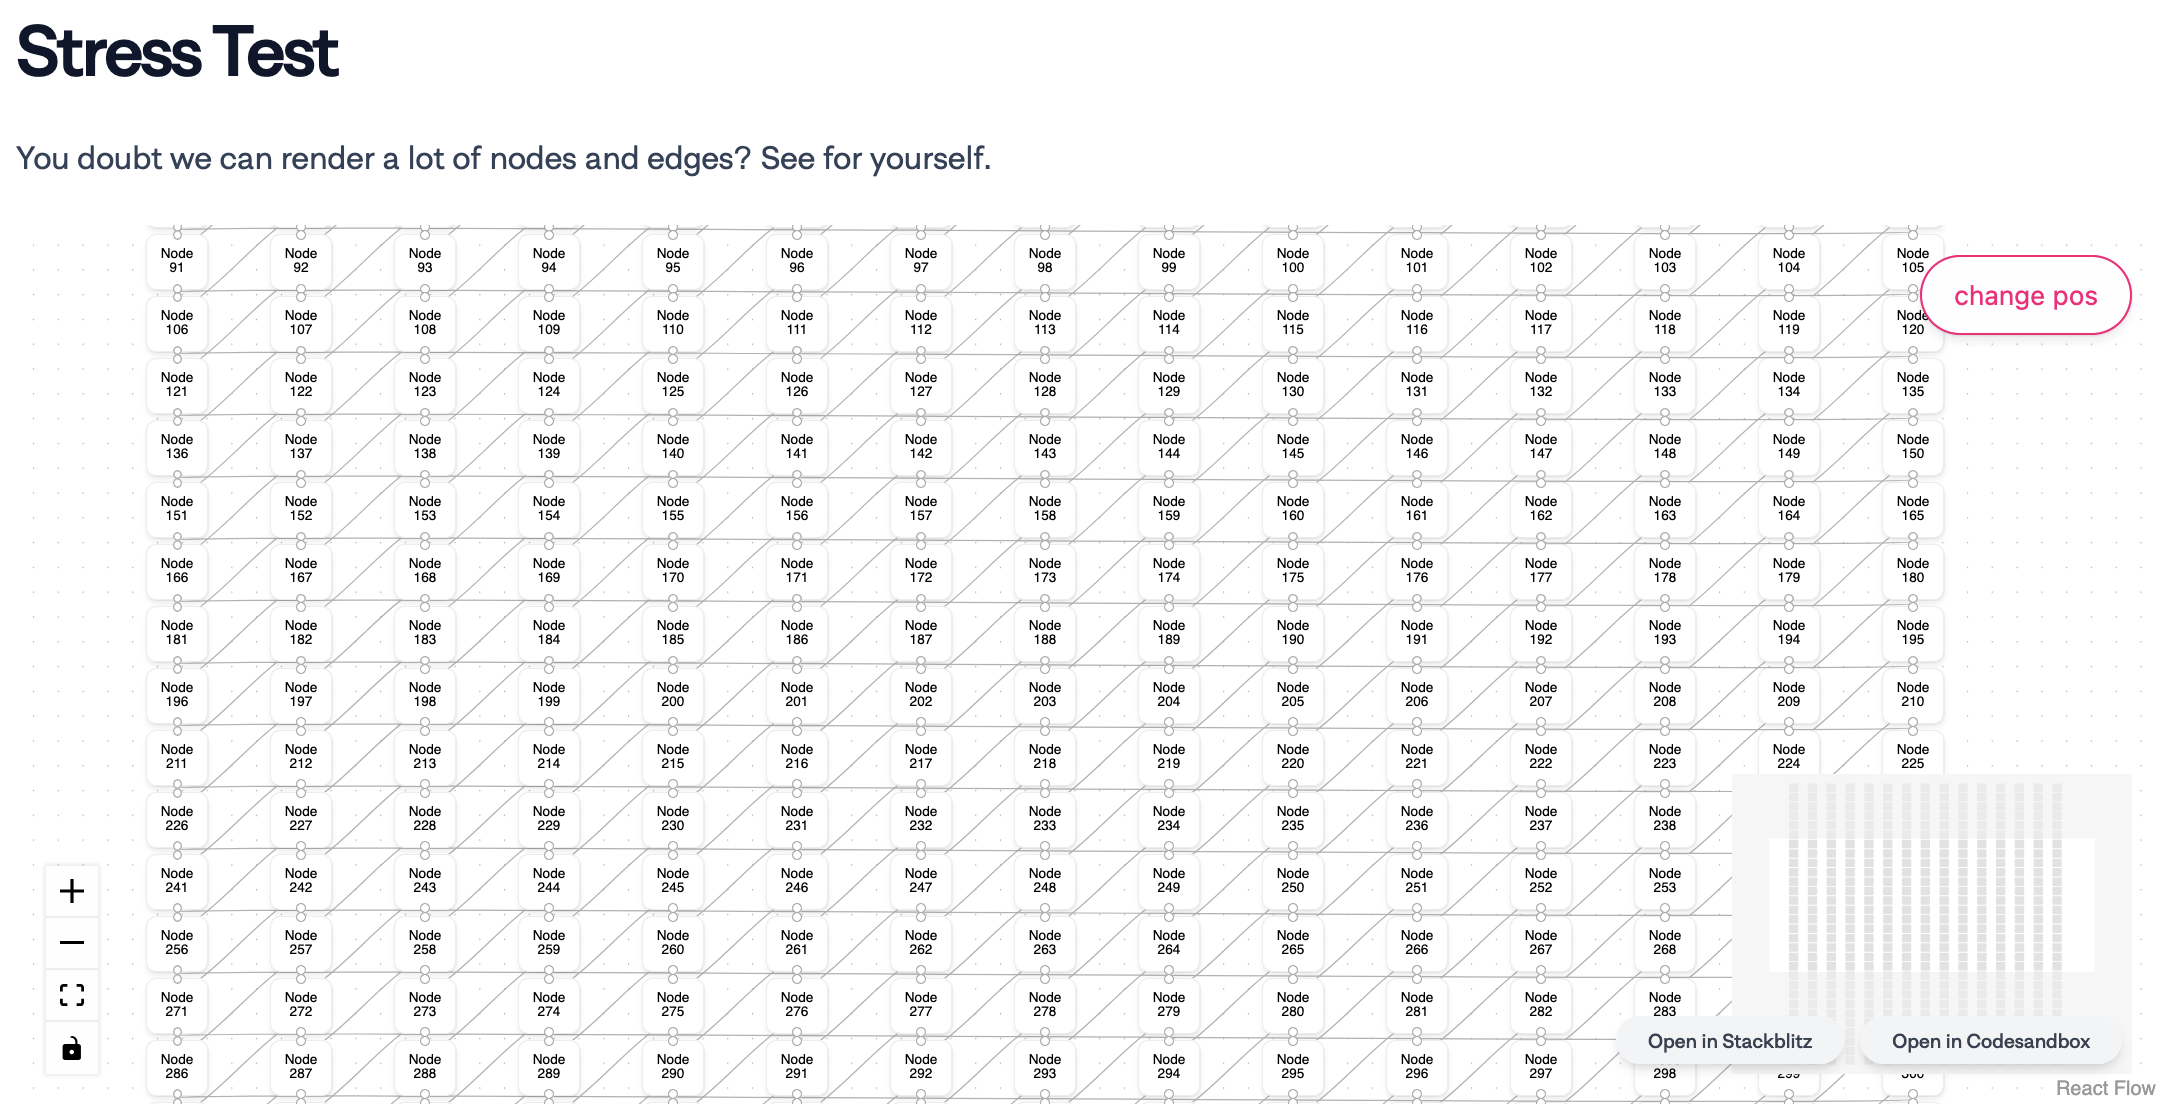
\includegraphics[width=0.85\textwidth]{img/stress-test.png}
  \caption{Stress test de ReactFlow affichant plusieurs centaines de nœuds}
\end{figure}
\noindent
Plusieurs optimisations ont donc été mises en place dans l’application. Tout d’abord, l’option de rendu conditionnel des nœuds a été activée : seuls les nœuds visibles à l’écran sont effectivement rendus et calculés par ReactFlow, tandis que ceux situés en dehors du champ de vision sont temporairement ignorés. Cette approche permet de réduire significativement la charge de calcul lors du rendu du canvas, en évitant de traiter inutilement des éléments invisibles pour l’utilisateur.
\\\\
Ensuite, la gestion de la sauvegarde automatique des modifications a été revue. Initialement, chaque modification sur le canvas (déplacement, ajout ou suppression de nœud) déclenchait une sauvegarde immédiate, ce qui pouvait saturer le serveur et ralentir l’interface. Pour remédier à cela, une fonction de sauvegarde « debounce » a été implémentée : les sauvegardes ne sont effectuées qu’après un court délai d’inactivité, ce qui permet de regrouper plusieurs modifications successives en une seule opération. Cette technique allège considérablement la charge sur le backend et améliore la réactivité globale de l’application.
\\\\
Grâce à ces ajustements, il a été possible d’assurer une expérience utilisateur fluide, même lors de la manipulation de thématiques complexes et très denses en compétences.
\subsubsection{Évolutions des besoins}
Beaucoup de demande qui ne pouvait pas être réalisé avec l'architecture actuelle

+ Demande de création de version

+ Demande de création d'exportation etc...
\subsubsection{Propreté du code}
Parler de sonarqube

Dire que apprendre en développant le projet est compliqué pour avoir quelque chose de propre dès le début car c'est dur de savoir dans quelle direction on va.

\subsection{Tests et validation}
\subsubsection{Types de tests}
Test unitaires avec jest
+ Installation en cours de test E2E (End to End) avec Playwright
\subsubsection{Retours utilisateurs}

\section{Retour d’expérience, prise de recul et conclusion}

\subsection{Compétences développées}
\subsubsection{Compétences techniques}
\subsubsection{Compétences méthodologiques}
\subsubsection{Compétences personnelles}

\subsection{Comparaison grande/petite entreprise}
\subsubsection{Environnement de travail}
\subsubsection{Encadrement et autonomie}
\subsubsection{Organisation des projets}

\subsection{Axes d’amélioration personnelle}
\subsubsection{Choix techniques}
\subsubsection{Gestion de projet}
\subsubsection{Organisation personnelle}

\subsection{Impact du projet chez Niji}
\subsubsection{Utilisation actuelle}
\subsubsection{Retours internes}
\subsubsection{Perspectives d’évolution}

\subsection{Perspectives professionnelles}
\subsubsection{Suite de parcours}
\subsubsection{Réflexions sur le domaine d’activité}

\subsection{Conclusion générale}

\section{Annexes}


\end{document}
